\documentclass[a4paper,twocolumn,10pt]{article}
\usepackage[spanish]{babel}
\usepackage[T1]{fontenc}
\usepackage[utf8]{inputenc}
\spanishdecimal{.}
\usepackage{lmodern}
\usepackage[a4paper]{geometry}
\usepackage{graphicx}
\usepackage{flushend}
\usepackage{wallpaper}
\usepackage{amsmath}
\usepackage{float}
\usepackage{colortbl}

\begin{document}

\title{Experimentos con microondas}
\author{ \\Aldo Aliaga, Benjamín Yapur, Fabian Trigo \\ \textit{Departamento de Física y Astronomía, Universidad de Valparaiso}}
\twocolumn[
  \begin{@twocolumnfalse}
    \maketitle
    \begin{abstract}
    
    \end{abstract}
  \end{@twocolumnfalse}\bigskip]

\vspace{2cm}

\section{Introducción}

Las microondas son un tipo de radiación electromagnética con longitudes de onda que van desde un metro a un milímetro, correspondientes al rango de frecuencias entre $300[MHz]$ y $300[GHz]$. Su naturaleza ondulatoria le otorga las propiedades de reflexión, refracción difracción e interferencia. 

Se puede conocer la frecuencia de las microondas emitidas relacionando su longitud de onda con la velocidad de propagación de las ondas en el medio:
\begin{equation}
    f=\frac{c}{\lambda}
\end{equation}


\section{Montaje}

Primeramente se realiza el montaje del sistema de guías, conformado de dos rieles y un plato graduado con una montura para el portaplacas.

Se cuenta con una antena de bocina emisora y una receptora. Estas se orientarán en el sistema de guías de acuerdo a cada experimento.

También se utiliza una fuente de poder en la cual se pude regular la amplificación de la señal, conectar las bocinas y conectar un voltímetro para medir la intensidad de la señal.

A continuación se detalla el montaje para cada experiencia:

\subsection*{1 Propagación Lineal del Microondas}
Detector frente al emisor
\begin{figure}[H]
    \centering
    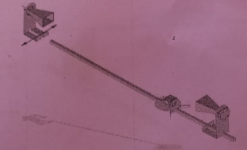
\includegraphics{MO_montaje/1.png}
    \caption{Montaje del experimento de propagacion lineal del microondas}
    \label{fig:proplineal}
\end{figure}

\subsection*{2 Poder de Penetración}

\begin{figure}[H]
    \centering
    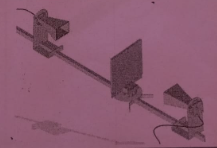
\includegraphics{MO_montaje/2.png}
    \caption{Montaje del experimento del poder de penetracion}
    \label{fig:montpen}
\end{figure}

\subsection*{3 Apantallamiento y Absorcion}
Utilizando dos materiales distintos se mide el cambio de intensidad con cada uno, uno es amde
\begin{figure}[H]
    \centering
    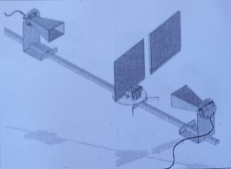
\includegraphics{MO_montaje/3.png}
    \caption{Montaje del experimento que comprueba apantallamiento y absocion}
    \label{fig:montapant}
\end{figure}

\subsection*{4 Reflexion}

\begin{figure}[H]
    \centering
    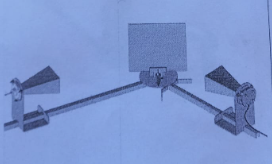
\includegraphics{MO_montaje/4.png}
    \caption{Experimento de reflexion}
    \label{fig:montreflex}
\end{figure}

Con emisor/receptor en un angulo de 90 grados a la misma distancia de 200 milimetros del centro, se controla la normal de la pantalla conductora, la cual funciona como reflector.

\subsection*{5. Onda Estacionaria, Longitud de Onda}
\begin{figure}[H]
    \centering
    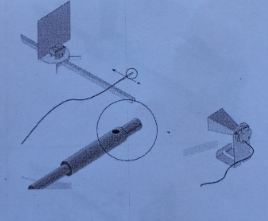
\includegraphics{MO_montaje/5.png}
    \caption{Caption}
    \label{fig:my_label}
\end{figure}

\subsection*{6. Refraccion}
Este experimento fue omitido por recomendacion del profesor y solo sera listado su construccion, pero no aparecera en el analisis
\begin{figure}[H]
    \centering
    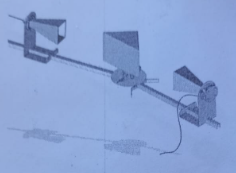
\includegraphics{MO_montaje/6.png}
    \caption{Refraccion con material}
    \label{fig:montrefr}
\end{figure}

\subsection*{7. Principio de Hyugens}
\begin{figure}[H]
    \centering
    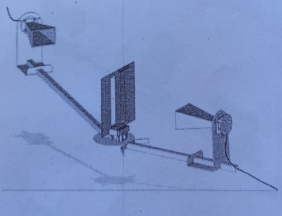
\includegraphics[scale=.7]{MO_montaje/7.png}
    \caption{Montaje experimento principio de Hyugens}
    \label{fig:hyu}
\end{figure}

\subsection*{8. Difracción}
Utilizando un sensor se mide la intensidad atravez de dos rendijas
\begin{figure}[H]
    \centering
    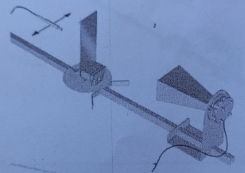
\includegraphics{MO_montaje/8.png}
    \caption{Experimento de difraccion}
    \label{fig:montdif}
\end{figure}

\subsection*{9. Interferencia}
Se colocan un rendija simple y una rendija doble en el soporte portaplacas, con la bocina emisora a 12 (cm) de la placa y la sonda receptora unos 6 (cm) de la de la placa. La sonda es desplazada en línea recta por un eje paralelo a la placa.
\begin{figure}[H]
    \centering
    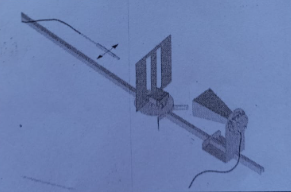
\includegraphics[scale=.7]{MO_montaje/9.png}
    \caption{Montaje experimento 9.}
    \label{fig:montinter}
\end{figure}

\subsection*{10. Polarizacion}
Se enclava la rendija de polarización en el portaplacas a 250 (mm) de las bocinas. Primero de forma vertical, luego horizontal y finalmente en diagonal. Se mide la intensidad de la señal para cada caso y también rotando las bocinas en 45 y 90 grados.
\begin{figure}[H]
    \centering
    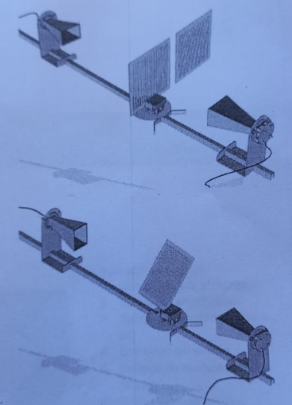
\includegraphics[scale=.7]{MO_montaje/10.png}
    \caption{Montaje del experimento de polarizacion}
    \label{fig:montpol}
\end{figure}





\section{Análisis}
Gran parte de los experimentos son de caracter cualitativo, aquellos numericos se proporcionara una tabla con los datos, el primer paso para analizar, fue apagar todo emisor y medir el voltaje del receptor, un voltaje base de $0.37 [V]$ considerado como el voltaje de ruido, por tanto cada vez que se tenga un voltaje cercano a este puede considerarse 0.

\subsection*{1 Propagacion Lineal del Microondas}
Frente a frente tienen una intensidad de $3.16 [V]$, osea en $0$ grados, de aqui en adelante se listara en una tabla:
\begin{table}[H]
\centering
\caption{Intensidad vs el angulo del receptor referente al emisor}
\begin{tabular}{rr}
\rowcolor[rgb]{0.753,0.753,0.753} \multicolumn{1}{l}{angulo [grad]} & \multicolumn{1}{l}{intensidad [V]}  \\
0                                                                   & 3.16                                \\
10                                                                  & 2.75                                \\
15                                                                  & 2.43                                \\
20                                                                  & 1.96                                \\
25                                                                  & 1.3                                 \\
30                                                                  & 0.75                                \\
35                                                                  & 0.5                                 \\
40                                                                  & 0.4                                
\end{tabular}
\end{table}

Se observa que decae conforme el angulo se aleja, osea, la onda se mueve de manera lineal.

\subsection*{2 Poder de Penetracion}
El voltaje con la amplitud del aparato, en linea recta y sin nada en su camino, fue de: $4.87 [V]$
En el caso de tener un obstaculo de madera, el voltaje: $4.37 [V]$ osea se apantalla levemente;

\subsection*{3 Apantallamiento y Absorcion}
El voltaje con la amplitud del aparato, en linea recta y sin nada en su camino, fue de: $4.87 [V]$
mientras que con un conductor en su camino: $0.39 [V]$, deciende al nivel del rudio del aparato, considerado como 0

Sumando una placa de madera, seca u humedecida disminuyo a $0.37 [V]$
\subsection*{4 Reflexión}
Con la normal de la pantalla metalica (reflector) en un angulo de 60 grados relativo al 0 del receptor, el voltaje fue de $1.63 [V]$, hasta que a los 45 grados se obtuvo el maximo: $4.61 [V]$.
Sigue a la perfeccion la ley de reflexion para las ondas.

\subsection*{5. Onda Estacionaria, Longitud de Onda}
Con mucho cuidado y la amplitud del emisor a la mitad para tener mas intensidad, los maximos:
\begin{table}[H]
\centering
\caption{Maximos registrados en un intervalo, para el calculo de $\lambda$}
\begin{tabular}{rr}
\rowcolor[rgb]{0.753,0.753,0.753} \multicolumn{1}{l}{Distancia [mm]} & \multicolumn{1}{l}{intensidad [V]}  \\
346                                                                  & 3.95                                \\
315                                                                  & 3.46                               
\end{tabular}
\end{table}

de esa manera la longitud de onda $\lambda$:
$$
\lambda = 346 - 315 = 31 [mm]
$$
Luego reemplazando para comparar con la frecuencia del aparato ($9.3 [GHz]$)
$$
f = \frac{c}{\lambda} [\frac{m/s}{m}] = 9.67 [GHz]
$$
Con tan solo un error de $9.67 - 9.3 [GHz] = 0.37 [GHz]$

\subsection*{7. Principio de Hyugens}
Se observo que el angulo donde consigue llegar señal ahora es mayor, producto de que la rendija funciona como un nuevo origen de la onda. Queda asi comprobado el principio de Hyugens.

\subsection*{8. Difracción}
Al mover el detector por detrás, se registra un incremento de intensidad cerca de los bordes, pero una vez en el centro (tras la pantalla conductora que no permite pasar las ondas), la intensidad decae bruscamente y vuelve a elevarse al aproximarse al borde sin aun mirar directamente al emisor. 
Quedo asi vista la difraccion, pues la onda se comporta de manera similar a si volviera a generarse en los bordes.

\subsection*{9. Interferencia}
Al desplazar la sonda se registra la intensidad de la emisión con respecto al tiempo, mostrando mayor intensidad cuando la sonda está frente a la rendija. 
\begin{figure}[H]
    \centering
    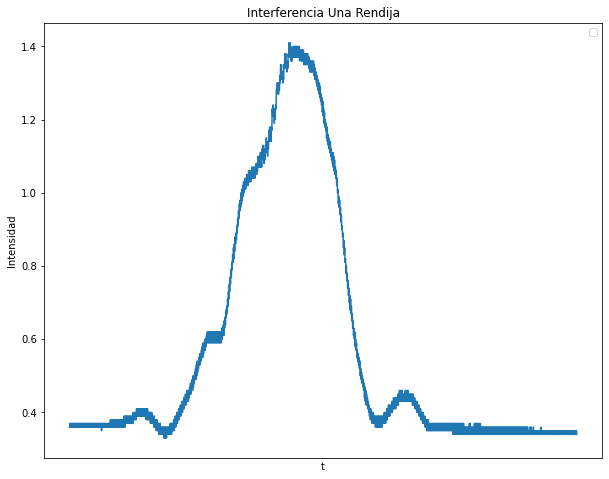
\includegraphics[scale=.3]{PlotMOAnalisis/plot_una_rendija.png}
    \caption{Intensidad en función del tiempo a través de una rendija.}
    \label{fig:my_label}
\end{figure}

En la figura 10 se aprecia dicha relación para la rendija simple. De ella se puede apreciar un peak  central que representa el momento en que no hay interferencia entre la sonda y la bocina emisora, es decir, cuando está justo en frente de la rendija. Además se ven dos peaks menores a cada lado separados por dos valles del peak central, pero como hay interferencia en esos sectores, se asocian estos peaks a la superposición de las ondas difractadas por la rendija.
\begin{figure}[H]
    \centering
    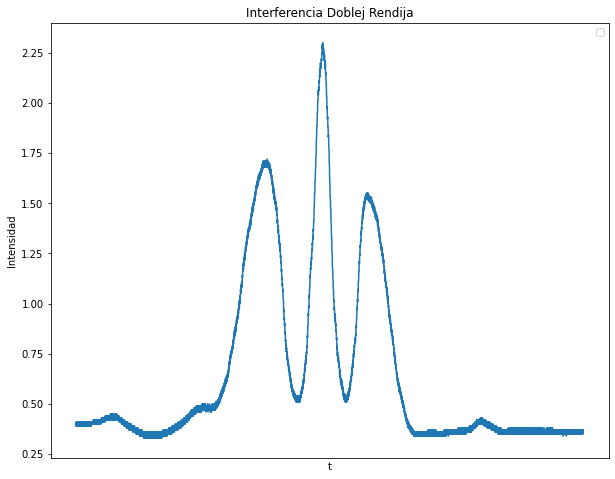
\includegraphics[scale=.3]{PlotMOAnalisis/plot_doble_rendj.png}
    \caption{Intensidad en función del tiempo a través de una doble rendija.}
    \label{fig:my_label}
\end{figure}

En la figura 11 se aprecian tres peaks y dos laterales, siguiendo el mismo patrón gaussiano. Estos peaks y valles también se deben por la difracción producida por las rendijas y la interferencia de estas ondas difractadas.

Ambos patrones corresponden los de difracción e interferencia de las ondas electromagnéticas.



\subsection*{10. Polarización}
Primero se mide la el voltaje cuando el sistema está apagado y prendido sin \textit{ningún dispositivo que interfiera}, registrando 0.37[V] y 6.73[V] respectivamente. El hecho de que se reciba señal incluso cuando la emisión está apagada es debido al ruido de fondo. Mientras que si la bocina emisora es rotada 90° la intensidad disminuye a 0.77[V]. Este resultado indica que las microondas tienen una mayor amplitud en el eje vertical que en el horizontal.

Al tener el polarizador de forma \textit{vertical} sin rotar la bocina emisora se obtiene una intensidad de 0.55[V]. Mientras que al rotar la bocina emisora se obtiene 0.37[V]. De estos resultados es claro que el voltaje disminuye considerablemente en ambos casos, del primero de ellos se puede extraer que las microondas son horizontales cuando no se rota la bocina. Por ende la disminución del voltaje se debe netamente a la rejilla polarizadora. En el segundo resultado el polarizador terminó de suprimir las ondas (ahora verticales) que podían ser recibidas por la bocina receptora, anulando por completo la señal.

Posicionando el polarizador de forma \textit{horizontal} sin rotar la bocina emisora se mide 6.63[V]. Y al rotar la bocina se registra 0.37[V]. A partir del primer resultado se puede decir que el polarizador en esta posición solo disminuye en un $1.48\%$ el voltaje.
De este primer resultado las ondas verticales (predominantes) pasan por el polarizador, mientras que las horizontales son sustraídas por la placa.
El segundo resultado es el mismo caso que para el polarizador en forma vertical.

Luego se posicionó el polarizador en 45° 


\section{Conclusión}

\newpage
\section{Bibliografía}


\begin{itemize}
\item
\end{itemize}


\end{document}